\chapter{Electrostatic equation -- Computation of fringe capacitance}

\modinfo{Directory}{FringeCapacitance}
\modinfo{Solvers}{\Idx{StatElecSolver}}
\modinfo{Tools}{\Idx{ElmerGUI}}
\modinfo{Dimensions}{2D, Steady-state}
\modinfo{Author}{Peter R{\aa}back}


\subsection*{Case definition}

This case presents solving the Laplace equation for electric potential.
\begin{equation}
  - \nabla \cdot \varepsilon \nabla \phi = 0  \, \, \, \, \in \, \, \Omega
\end{equation}
where the electric potential $\phi$ is given at conducting surfaces.
This is a standard type of equation with many variants in physics, electrostatics being just one of them.
From the solution one may calculate 
derived fields, and 
\Idx{capacitance}
which is obtained from the total electric energy 
\begin{equation}
  E=\frac{1}{2} \int \varepsilon | \nabla \phi |^2 \, d\Omega
\end{equation}
and the relation $E=CU^2/2$.

\begin{figure}[h]
\centering
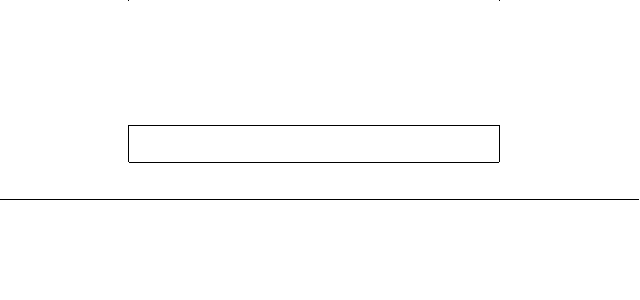
\includegraphics[width=10cm, viewport=0 20 640 280,clip]{capacitor}
\caption{The geometry of the capacitor}\label{fg:es_capacitor}
\end{figure} 

The geometry studied 
is a 2D plate capacitor having the well known approximation
for Capacitance $C_{app}=\varepsilon_r\varepsilon_0 A/d$.
With the help of the
simulation one may evaluate the fringe capacitance resulting
from the end effects of the capacitor geometry.
The measurements of the capacitor are $10 \times 1$, and the distance to
ground is also 1. Defining the permittivity of vacuum to be 
$\epsilon_0 = 1$ the comparison to the analytical approximation
becomes trivial since then then $C_{app} = 10$. 

The derived fields in the StatElecSolver are computed 
by averaging the fields over elements -- not using the 
Galerkin method which would provide optimal accuracy. The fields 
may, however, be sufficient for visualization purposes. 



\begin{figure}[h]
\centering
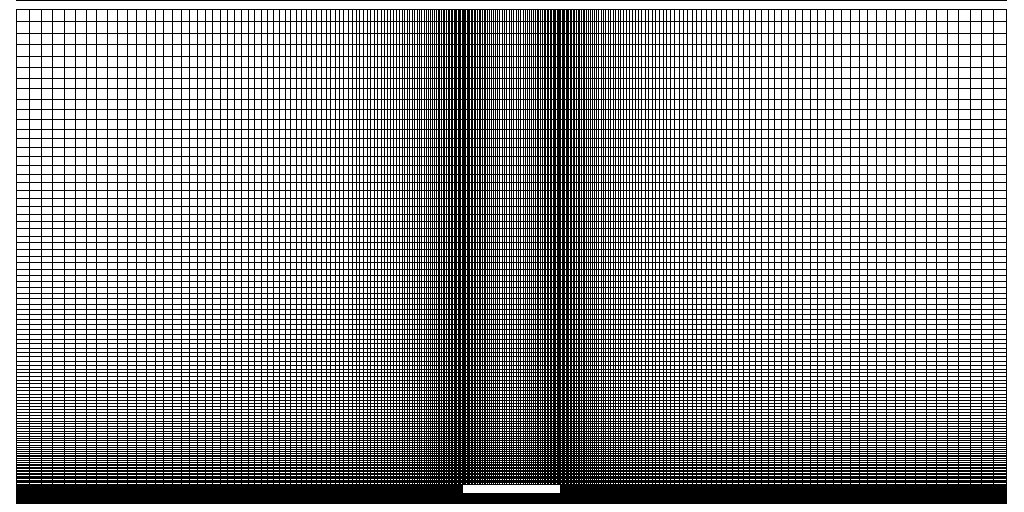
\includegraphics[width=120 mm]{mesh}
\caption{Computational mesh used in the simulation}\label{fg:es_geometry}
\end{figure}  




\subsection*{Solution procedure}

The definitions for the electrostatic equation are not loaded into ElmerGUI by default. Hence, 
one needs to load these before starting the simulations.
\ttbegin
File 
  Definitions
    Append -> electrostatics.xml
\ttend
The additional definitions should reside in the directory \texttt{edf-extra} within the distribution.
Moving the desired \texttt{xml} files to the \texttt{edf}-directory enables automatic loading of the 
definitions at start-up. By inspecting the definitions in the \texttt{Elmer Definitions File editor} one
may inspect that the new definitions were really appended. 


The mesh is given in ElmerGrid format in file \texttt{disc.grd}, load this file.
\ttbegin
File 
  Open -> disc.grd
\ttend
You should obtain your mesh and may check that it consists of 30484 nodes and of 30348 bilinear elements.


After we have the mesh we start to go through the Model menu from the top to bottom. 
In the Setup we choose things related to the whole simulation such as file names, 
time stepping, constants etc.
The steady-state simulation is carried out in 2-dimensional Cartesian
coordinates. For convenience we also set $\varepsilon$ equal to one. 
\ttbegin
Model
  Setup 
    Simulation Type = Steady state
    Vacuum Permittivity = 1.0
\ttend
In the equation section we choose the relevant equations and parameters related to their solution. 
In this case we'll have only the electrostatics solver. 

When defining Equations and Materials it is possible to assign to the bodies immediately, or to use mouse
selection to assign them later. In this case we have just one body and therefore its easier to assign 
the Equation and Material to it directly.

In the solver specific options we want to activate some flags that are needed to invoke the 
computation of derived fields. 
For the linear system solvers we are happy to use the defaults. One may however, try out different
preconditioners (ILU1,\ldots) or direct Umfpack solver, for example.
\ttbegin
Model
  Equation
    Name = Electrostatics
    Apply to Bodies = 1
    Electrostatics
      Active = on
      Edit Solver Settings
        Solver specific options
          Calculate Electric Field = True
          Calculate Electric Energy = True
    Add 
    OK
\ttend        
The Material section includes all the material parameters.
In this case we only have the relative permittivity which we set to one.
\ttbegin
Model
  Material
    Name = Ideal
    Electrostatics
      Relative Permittivity = 1.0
    Apply to Bodies = 1 
    Add
    OK
\ttend

We have two boundary conditions for the potential at the ground and at the capacitor. For other boundaries
the do-nothing boundary results to zero flux over the boundary.
\ttbegin
Model
  BoundaryCondition
    Name = Ground
    Electrostatics
      Potential = 0.0
    Add
    New

    Name = Capacitor
    Electrostatics
      Potential = 1.0
    Add
\ttend   

The conditions may also be assigned to boundaries in the Boundary condition menu, or 
by clicking with the mouse. Here we use the latter approach as that spares us of the 
need to know the indexes of each boundary.
\ttbegin
Model
  Set boundary properties
    Choose Ground -> set boundary condition Ground
    Choose Capacitor -> set boundary condition Capacitor
\ttend


For the execution 
ElmerSolver needs the mesh files and the command file. We have now basically defined
all the information for ElmerGUI to write the command file. After writing it we may also visually 
inspect the command file.
\ttbegin
Sif 
  Generate
  Edit -> look how your command file came out  
\ttend

Before we can execute the solver we should save the files in a directory. The project includes
all the files needed to restart the case.
\ttbegin
File 
  Save Project
\ttend

After we have successfully saved the files we may start the solver
\ttbegin
Run
  Start solver
\ttend
A convergence view automatically pops up showing relative changes of each iteration.
The equation is fully linear and hence only two iterations are needed -- the second 
one just ensures that convergence of the non-linear level was really obtained. 
The norm of the solution should be 0.3055.

When the solution has finished we may start the postprocessor to view some results.
\ttbegin
Run
  Start ParaView
\ttend


\subsection*{Results}

From the output of the simulation one may see that the 
capacitance in this case was 13.697 compared to the analytical estimate of 10. 
Hence the fringe capacitance in this case increases the capacitance by 37~\%. 

\begin{figure}[h]
\centering
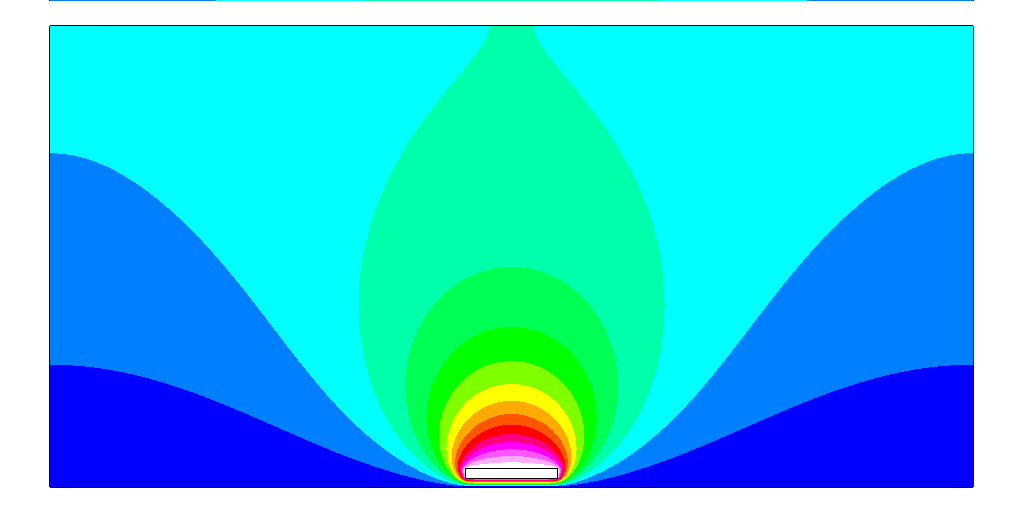
\includegraphics[width=10cm, viewport=0 20 1024 480,clip]{potential}
%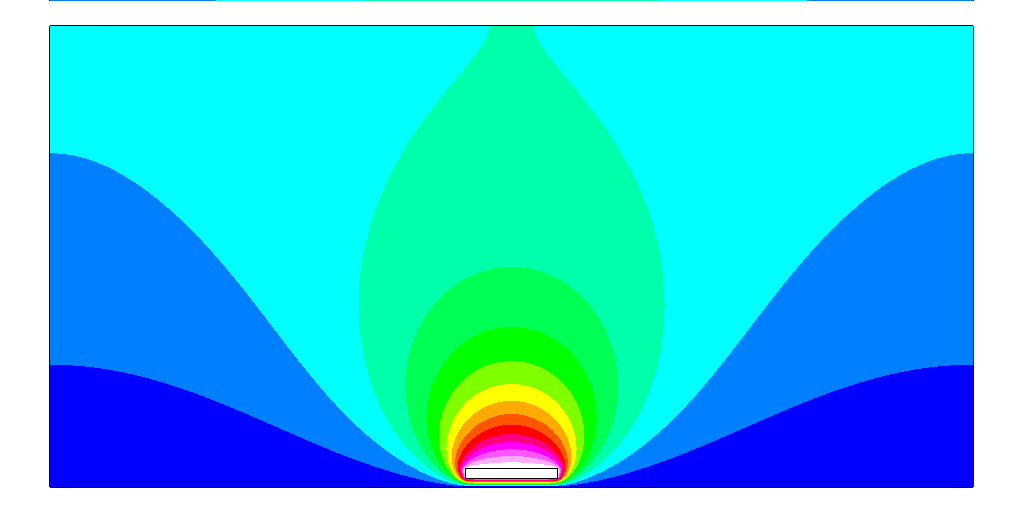
\includegraphics[width=12cm]{potential}
\caption{The electrostatic potential}\label{fg:es_potential}
\end{figure} 

\begin{figure}[h]
\centering
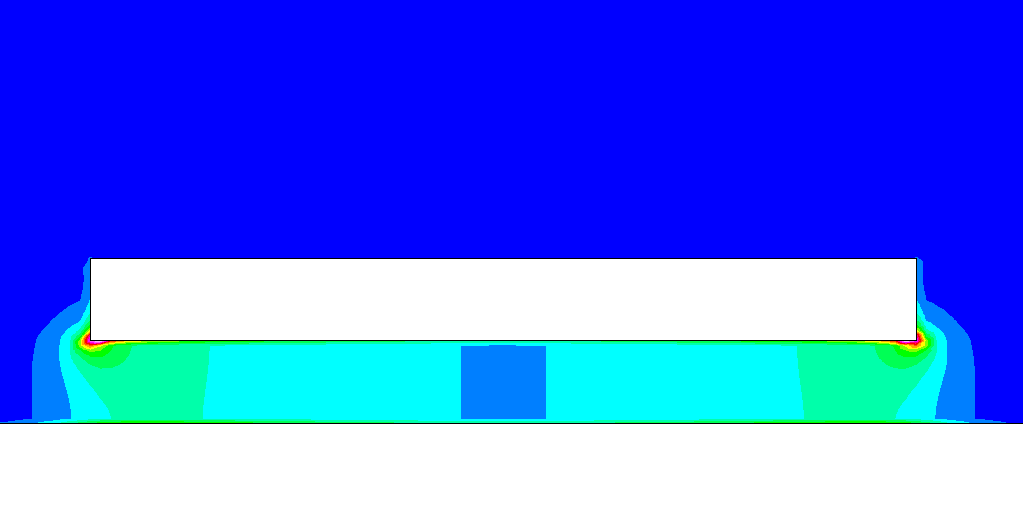
\includegraphics[width=9cm, viewport=0 20 1024 480,clip]{energy}
%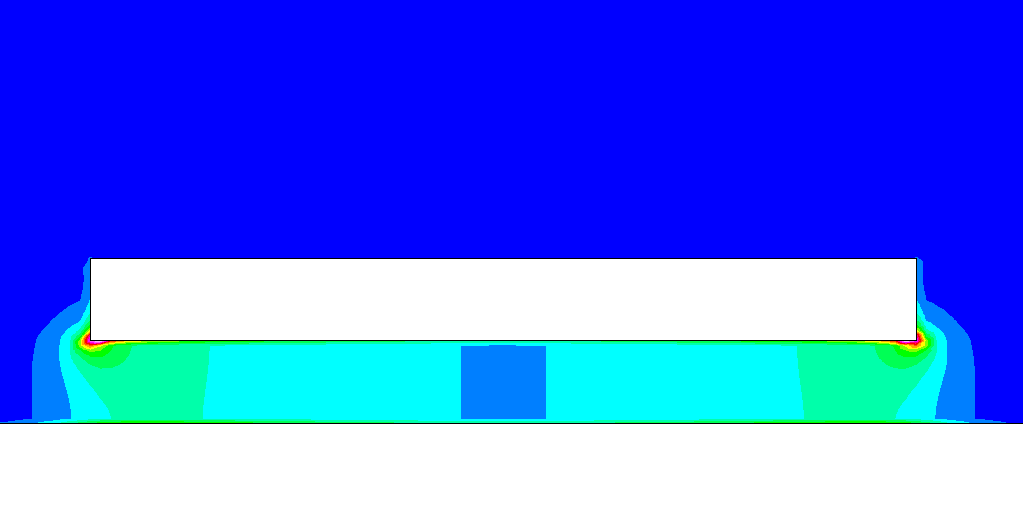
\includegraphics[width=12cm]{energy}
\caption{The electrostatic energy density, a close-up}\label{fg:es_energy}
\end{figure} 


\hfill

